The general second order equation is given by ,
\begin{align}
ax^2+2bxy+cy^2+2dx+2ey+f&=0\label{eq:solutions/13/ex1/eq1}
\end{align}
Given,
\begin{align}
    12x^2+7xy-10y^2+13x+45y-35&=0 \label{eq:solutions/13/ex1/eqgiven}
\end{align}
The above equation can be expressed as
\begin{align}
        \vec{x}^{T}\vec{Vx} + 2\vec{u}^{T}\vec{x} + f=0   \label{eq:solutions/13/ex1/eq:solutions/eq2}
\end{align}
where
\begin{align}
	\vec{V}=\vec{V}^T &= \myvec{12 & \frac{7}{2} \\ \frac{7}{2} & -10} \\
	\vec{u} &= \myvec{\frac{13}{2} \\ \frac{45}{2}} \\
	 f=-35
\end{align}	
	(\ref{eq:solutions/13/ex1/eq:solutions/eq2}) represents a pair of straight lines if
\begin{align}
	&\mydet{\vec{V} & \vec{u} \\ \vec{u}^T & f} = 0     \label{eq:solutions/13/ex1/eq:solutions/eq5} \\
	\mydet{\vec{V} & \vec{u} \\ \vec{u}^T & f} 
		&= \mydet{12 & \frac{7}{2}  & \frac{13}{2} \\ 
	        \frac{7}{2} & -10 & \frac{45}{2}     \\
	       \frac{13}{2} & \frac{45}{2} & -35 }  \\
	       		\nonumber \\
	\implies \ 12\mydet{-10 & \frac{45}{2} \\ \frac{45}{2} & -35} 
		& -\frac{7}{2}\mydet{\frac{7}{2} & \frac{45}{2} \\ \frac{13}{2} & -35} 
		+\frac{13}{2}\mydet{\frac{7}{2} & -10 \\ \frac{13}{2} & \frac{45}{2}} = 0 \label{eq:solutions/13/ex1/eq:solutions/eq10}
\end{align}
The lines intercept if
\begin{align}
        \mydet{\vec{V}} < 0 \\
 	\mydet{\vec{V}}=-\frac{529}{4} < 0 \label{eq:solutions/13/ex1/eq:solutions/eq11}
\end{align}
\renewcommand{\thefigure}{1}
From (\ref{eq:solutions/13/ex1/eq:solutions/eq10}) and (\ref{eq:solutions/13/ex1/eq:solutions/eq11}) it can be concluded that the given equation represents a pair of intersecting lines.\\
Let $(\alpha,\beta)$ be their point of intersection, then
\begin{align}
	\label{eq:solutions/13/ex1/eq16}\myvec{ 12 & \frac{7}{2}\\\frac{7}{2} & -10}\myvec{\alpha \\ \beta} = \myvec{\frac{-13}{2} \\ -\frac{45}{2}} \\
	\label{eq:solutions/13/ex1/eq17}\implies \myvec{\alpha \\ \beta} = \myvec{-1 \\ 2}
\end{align}
\begin{equation}
	\text{From \textit{Spectral theorem, }}\vec{V} = \vec{P}\vec{D}\vec{P}^T
\end{equation}
\begin{align}
	\label{eq:solutions/13/ex1/eq18}\vec{V} &= \myvec{ 12 & \frac{7}{2}\\ \frac{7}{2} & -10}\\
	\label{eq:solutions/13/ex1/eq19}\vec{P} &= \myvec{\frac{-\sqrt{533} - 22}{2} & \frac{-22 + \sqrt{533}}{2}\\ 1 & 1}\\
	\label{eq:solutions/13/ex1/eq20}\vec{D} &= \myvec{1 + \frac{\sqrt{533}}{2} & 0\\ 0 & 1 - \frac{\sqrt{533}}{2}}
\end{align}
Using \textit{Spectral decomposition} of matrix we can express equation as
\begin{align}
	\label{eq:solutions/13/ex1/eq14}u_1(x-\alpha) + u_2(y-\beta) &= \pm \sqrt{-\frac{\lambda_2}{\lambda_1}}(v_1(x-\alpha) + v_2(y-\beta))
\end{align}
Substituting values in above equation we get;
\begin{multline}\label{eq:solutions/13/ex1/eq21}
	\frac{\sqrt{533}-22}{2}(x+1) + (y-2) \\= \pm \sqrt{-\frac{1 - \frac{\sqrt{533}}{2}}{1 + \frac{\sqrt{533}}{2}}}\left(\frac{-22 -\sqrt{533}}{2}(x+1) + (y-2)\right)
\end{multline}
Simplifying \eqref{eq:solutions/13/ex1/eq21},
\begin{align}
	\label{eq:solutions/13/ex1/eq22}3x -2y + 7 = 0 \text{ and } 4x + 5y -5 = 0\\
	\implies (3x - 2y + 7)(4x + 5y - 5) = 0
\end{align}
Thus the equation of lines are
\begin{align}
	\myvec{4 & 5}\vec{x} = 5 \\
	\myvec{3 & -2}\vec{x} = -7 
\end{align}
\begin{figure}[h]
    \centering
    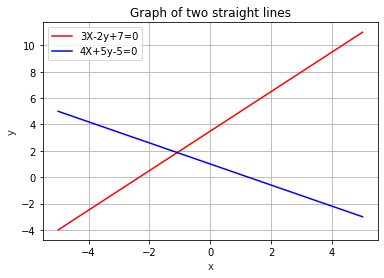
\includegraphics[width=\columnwidth]{./solutions/13/ex1/Figure.png}
    \caption{Pair of straight lines}
    \label{eq:solutions/13/ex1/Fig :1}
\end{figure}
{Angle between the straight lines: }
The angle between the lines can be expressed in terms of normal vectors 
\begin{align}
	\vec{n_1}=\myvec{4\\5} , \quad \vec{n_2}=\myvec{3\\-2}
\end{align}
\begin{align}
	\cos\theta=\frac{\vec{n_1}^T\vec{n_2}}{\norm{\vec{n_1}}\norm{\vec{n_2}}} \\
				\nonumber \\
	\implies \quad \theta=\cos^{-1}({\frac{2}{\sqrt{533}}}) = \tan^{-1}(\frac{23}{2})
\end{align}
